
\documentclass[aspectratio=169,9pt]{beamer}

\usetheme{Madrid}
\usecolortheme{whale}
\usepackage{amsmath, amssymb}
\usepackage{booktabs}
\usepackage{xcolor}
\usepackage{tikz}
\usetikzlibrary{positioning}

\setbeamertemplate{navigation symbols}{}
\setbeamertemplate{footline}[frame number]
\setbeamerfont{block body}{size=\small}
\setbeamerfont{block title}{size=\small}

\newcommand{\nn}{\texttt{n}}
\newcommand{\uu}{\texttt{u}}
\newcommand{\eq}{\texttt{=}}
\newcommand{\hwt}{\mathrm{H}}
\newcommand{\bd}{\mathrm{BD}}
\newcommand{\xor}{\oplus}
\newcommand{\badd}{\boxplus}
\newcommand{\bsub}{\boxminus}
\definecolor{key}{rgb}{0.0,0.35,0.0}
\definecolor{hot}{rgb}{0.70,0.0,0.0}
\newcommand{\key}[1]{\textcolor{key}{\textbf{#1}}}
\newcommand{\hot}[1]{\textcolor{hot}{#1}}

\title[SAT/SMT collision attacks on SHA-2]{SAT/SMT Based Differential Cryptanalysis of SHA-2}
\subtitle{Difference modelling, Bit Conditions and Objective Minimization }
\author{}
\date{\today}

\begin{document}

\begin{frame}\titlepage\end{frame}

% =====================================================================
\begin{frame}{Index}
\begin{enumerate}\small
  \item \textbf{The idea:} SMT-modelled search for high-probability DCs.
  \item \textbf{Reading a DC:} an example characteristic; where the \texttt{0}/\texttt{1} pins come from; how operations are modelled.
  \item \textbf{Two models} (difference vs.\ value); determinism; where contradictions slip by; what the value model fixes.
  \item \textbf{2024 (Li--Liu--Wang):} Hamming-weight-only objective $+$ a proof that for modular addition this is \emph{exactly} the condition count.
  \item \textbf{2025 (Li et al., CRYPTO):} Hamming weight $+$ 2-bit conditions; but an over-counting objective.
  \item \textbf{2026 (Zhang--Li--Gao, main focus):} automated local-collision search $+$ a corrected, complete objective; pipeline $+$ our reproduction.
  \item \textbf{Message modification:} single-block (SFS) $\to$ two-block collision.
  \item \textbf{Further work.}
\end{enumerate}
\end{frame}

% =====================================================================
\section{The idea}

\begin{frame}{The idea: SMT-modelled search for high-probability DCs}
\begin{itemize}
  \item Encode each step operation (modular add, $\Sigma/\sigma$, IF, MAJ, expansion) as constraints on \key{signed differences}; hand to an SMT solver (STP $+$ CryptoMiniSat).
  \item A satisfying assignment $=$ a globally-consistent candidate DC.
  \item \key{Objective: minimize the number of bit conditions} (equivalently, maximize the DC's probability); work from 2024 minimizes Hamming weight; later work minimizes conditions directly.
\end{itemize}


\begin{block}{Signed difference $\nabla\kappa=(\kappa_v,\kappa_d)$}
\centering\small
$(0,0)=\eq$ free \;$(0,1)=\nn$ ($0\!\to\!1$) \;$(1,1)=\uu$ ($1\!\to\!0$)
\end{block}

\begin{alertblock}{Bit condition}
\small A constraint that \key{halves} the conforming-pair probability. Either occurs as a value-pin ($x=0$) or an (in)equality between two bits ($a=b$, $a\neq b$).
\end{alertblock}

\end{frame}

% =====================================================================
\section{Reading a DC}

\begin{frame}{What a differential characteristic is (example)}
 A DC is, per step $i$, the signed difference of each register: $\nabla A_i,\nabla E_i,\nabla W_i$; a per-bit string over $\{\eq,\nn,\uu\}$ plus value-pins $\{\texttt{0},\texttt{1}\}$. It shows step-by-step of how a particular difference is injected and propagated, for a collision to occur. 
 
\begin{block}{Excerpt; 37-step SHA-256 DC (Zhang et al.\ 2026, Table 8), steps 4--9}
\centering\ttfamily\footnotesize
\begin{tabular}{r l l l}
$i$ & $\nabla A_i$ & $\nabla E_i$ & $\nabla W_i$\\
4 & ================================ & =0=======11===1=========11=0==01 & ================================\\
5 & ================================ & =0====00110===0====1==0=11=1=101 & ================================\\
6 & ==n=======u===n==========n===u=u & 1nu=00110un00nu0=0=00=11nu0un0nn & nuu======un===n=========nu==un=u\\
7 & ================================ & 1n001=nnuu0=01u0n11u01u1uu110nun & ========nuuuuuuuuuuuuu===011====\\
8 & ================================ & nnn=10011nu0=0101=0011110=110n00 & ================================\\
9 & ================================ & 1=1===11111===0=1==1111110111110 & ====nuu=n======================n\\
\end{tabular}
\end{block}
\small \nn/\uu\ $=$ active (a flipped bit, with sign); \eq\ $=$ no difference, value free; \texttt{0}/\texttt{1} $=$ value is pinned.
\end{frame}

\begin{frame}{The \texttt{0}/\texttt{1} in the DC}
A \texttt{0}/\texttt{1} is a bit with \emph{no difference} but a \emph{forced value}. 
\begin{itemize}
  \item These are exactly the \key{bit conditions the nonlinear boolean gates require} for the chosen differences to propagate; imposed on otherwise difference-free bits.
  \item \emph{Example (IF):} the transition $\nabla(x,y,z,w)=[\eq\eq\nn\nn]$ propagates only if the selector $x[i]=0$ $\Rightarrow$ a \texttt{0} pin on a difference-free bit.
  \item  They can be read directly out of the per-transition condition tables. Their count is the exponent in the probability of differential characteristic.
\end{itemize}
\end{frame}

\begin{frame}{Modelling individual operations (modular addition example)}
\textbf{Method.} For each operation: (1) enumerate \emph{all valid} bit-level transitions over (input diffs, auxiliaries, output diff) into a truth table; (2) minimize to CNF (LogicFriday); (3) assert the CNF; the solver then only explores valid \emph{difference} transitions.
\begin{block}{Modular addition $z=x\badd y$ (per bit $i$)} Tuple of \key{signed differences}: $(\nabla x_i,\nabla y_i,\nabla c_i,\nabla z_i,\nabla c_{i+1})$ with a carry-difference $\nabla c$; $27$ valid transitions, e.g.
\[
\texttt{(}\eq,\eq,\eq,\eq,\eq\texttt{)},\quad \texttt{(}\nn,\eq,\eq,\nn,\eq\texttt{)},\quad \texttt{(}\nn,\eq,\eq,\uu,\hot{\nn}\texttt{)}\ \ldots
\]
A valid carry-difference chain $\Leftrightarrow$ a conforming value pair exists for that addition.
\end{block}
\begin{itemize}
  \item Each row $\to$ clauses over the input, auxiliary and output signed difference variables. The whole hash function is built by chaining these constrains on the specified variables.
  \item \textbf{Addition gates} have the input carry, output carry differences; aside from the inputs' $\nabla x_i, \nabla y_i$ differences. 
  \item \textbf{Boolean gates} additionally carry 3 \emph{monitor value bits} $(x,y,z)$ (auxiliary) in the tuple. In literature, usually referred to as the "full-model".
  \item The extra variables mentioned are the \emph{auxiliary} variables, which make the local transition \emph{deterministic}.
\end{itemize}
\end{frame}

% =====================================================================
\section{Two models}

\begin{frame}{Two models}
\begin{columns}
\begin{column}{0.5\textwidth}
\textbf{Difference model} (the search)
\begin{itemize}
  \item Variables: $(v,d)$ per bit $+$ auxiliaries (carry-diffs, value monitors).
  \item Per-operation propagation tables.
  \item Objective: sparsity $+$ conditions.
  \item Produces a \emph{candidate} DC.
\end{itemize}
\end{column}
\begin{column}{0.5\textwidth}
\textbf{Value model} (validity)
\begin{itemize}
  \item Real $n$-bit words, true $K_i$, full-adder carries.
  \item Each register's actual value is pinned to its signed-difference symbols.
  \item Decides whether a conforming pair \emph{exists}.
\end{itemize}
\end{column}
\end{columns}
\vspace{0.4em}
\begin{alertblock}{Why two models}
 The difference model is a \key{relaxation}: each operation asserts ``$\exists$ a value locally realizing the transition.''. However, local satisfiability for every piece $\not\Rightarrow$ global satisfiability. The gap is exactly the set of \key{invalid DCs}; the value model closes it.
\end{alertblock}
\end{frame}

\begin{frame}{Determinism of signed-difference propagation}
\begin{alertblock}{Deterministic Propagation}
If a given set of input signed differences yield a single $\nabla z$ such that \emph{every} conforming value pair yields it, i.e.\ $\Pr_{\text{conforming}}[\text{output}=\nabla z]=1$.
\end{alertblock}
\begin{itemize}
  \item \key{Deterministic:} NOT, shifts, rotations; output difference is fixed by the input difference.
  \item \key{XOR / $\Sigma,\sigma$:} activity deterministic, \emph{sign not}: $[\nn,\eq,\eq]\to$ active, but $\nn$ vs $\uu$ depends on the value of the inactive operand (two possible outputs).
  \item \key{IF / MAJ:} non-deterministic, e.g.\ a single $\nabla$-input can map to two $\nabla w$ depending on the hidden data bits.
  \item \key{Modular addition:} non-deterministic; one $(\nabla x,\nabla y)$ admits several $\nabla z$ via different carry behaviours.
\end{itemize}
\centering\emph{The non-deterministic transitions are made deterministic using auxiliary variables: carry-difference $\Delta c$ (addition) and monitor values (Boolean gates).}
\end{frame}

\begin{frame}{Contradictions missed by difference model: Value Model fixes}

DCs found by difference models are invalid since contradictions are missed.
\textbf{Root cause:} per-operation existential decoupling; ``$\exists$ a witness for me'' $\not\Rightarrow$ ``$\exists$ one trail-wide value-world.''
\begin{enumerate}
  \item \textbf{Value monitors untied to artihmetic:} $y_t$ is never forced to equal the value the additions actually compute for $E_t$. 
  \item \textbf{$K_i$ invisible} ($\Delta K_i=0$): only the value model uses it.
  \item \textbf{Modular-difference expansion is value-free:} a fixed modular difference has many signed representations; the solver may pick one no global assignment supports.
\end{enumerate}

These issues are fixed by pinning the signed differences at each step to the actual value bits, and contradictions will be yielded where no value bits can be found. However, the value model is \textbf{expensive}, and thus difference is used majorly, and value only for satisfying.

\end{frame}

% =====================================================================
\section{2024}

\begin{frame}{2024 (Li--Liu--Wang): a Hamming-weight-only objective}
\begin{itemize}
  \item First SAT/SMT tool for SHA-2 DCs; two coupled models (difference $+$ value).
  \item \key{Objective: minimize Hamming weight} of the signed differences (staged: $\sum\hwt(\nabla W)$, then $\sum\hwt(\nabla A)$, then $\sum\hwt(\nabla E)$).
  \item \key{Limitation:} Hamming weight ignores the bit conditions from the \emph{Boolean} functions $\Rightarrow$ the objective is \emph{not} the probability $\Rightarrow$ probabilities re-evaluated by hand.
\end{itemize}
\begin{block}{But Hamming weight is \emph{exactly} right for one part; modular addition}
 We can prove the number of bit conditions a modular addition imposes equals $\hwt(\nabla z)$ of its output. So the 2024 objective was \emph{optimal for the addition-induced conditions} and only \emph{blind to the Boolean ones}; exactly what 2025/2026 add.
\end{block}
\end{frame}

\begin{frame}{Proof: addition imposes exactly $\hwt(\nabla z)$ conditions (1/2)}
\small
$E_i$ is a sum of terms fixed \emph{outside} the addition, so the \key{modular difference $\delta z$ is forced} (value-independent). For a valid DC the chosen signed output $\nabla z$ is one representation of $\delta z$; its probability is
\[
\Pr[\nabla z] = \Pr_{z}\big[\pi(z)=\nabla z\big], \qquad \pi(z)=\text{signed diff of }(z,\,z\badd\delta z).
\]
With $z'=z\badd\delta z$, carry $\gamma$ ($\gamma_0=0$): $z'_i = z_i \xor \delta_i \xor \gamma_i$, $\gamma_{i+1}=\mathrm{MAJ}(z_i,\delta_i,\gamma_i)$, using $\mathrm{MAJ}(0,b,c)=b\wedge c$, $\mathrm{MAJ}(1,b,c)=b\vee c$. Per bit:
\begin{itemize}
  \item \textbf{inactive} ($\eq$): need $\delta_i=\gamma_i$, then $\gamma_{i+1}=\delta_i$; if $\delta_i\neq\gamma_i$ no $z$ works. \emph{No value bit fixed.}
  \item \textbf{active} ($\nn/\uu$): $\delta_i\xor\gamma_i=1\Rightarrow\gamma_i=1\xor\delta_i$ forced; the value bit is forced ($z_i=1$ for \uu, $0$ for \nn); $\gamma_{i+1}=z_i$.
\end{itemize}
\centering\emph{The whole carry trail is determined by $\nabla z$ alone; independent of the free values.}
\end{frame}

\begin{frame}{Proof: addition imposes exactly $\hwt(\nabla z)$ conditions (2/2)}
\small
\begin{itemize}
  \item Fixed value bits $=$ active bits $=\hwt(\nabla z)$; remaining $n-\hwt$ bits free, so $\#\{z\}=2^{\,n-\hwt(\nabla z)}$:
  \[
  \Pr[\nabla z]=2^{-\hwt(\nabla z)} \;\Longrightarrow\; \key{$\hwt(\nabla z)$ effective bit conditions, and no others.}
  \]
  \item These are exactly the self-pins ($\nn\!\to\!0$, $\uu\!\to\!1$); nothing else is hidden in the carries.
\end{itemize}
\begin{alertblock}{Why this needs \emph{signed} differences (the crux)}
\small For unsigned differences the count is \emph{not} $\hwt$: tracking the carry by start/continue/stop relations gives $\#\text{conditions}=\#\text{output differences}$, \key{minus one} for a contiguous run reaching the MSB (its carry-out is discarded). Signedness is what makes it exactly $\hwt$.
\end{alertblock}
\centering So the trail-search objective $\hwt(\nabla E_i)+\bd(E_i)$ is ``addition conditions ($\hwt$, exact) $+$ Boolean conditions ($\bd$),'' disjointly.
\end{frame}

% =====================================================================
\section{2025}

\begin{frame}{2025 (Li et al., CRYPTO): Hamming weight $+$ 2-bit conditions}
\textbf{2-bit condition:} a propagation constraint of the form $a=b$ or $a\neq b$ (two bits, one independent constraint).
\begin{alertblock}{Concrete motivation (XOR, in the signed paradigm)}
 $w=x\xor y\xor z$. Take $\nabla x=\nn$, $\nabla y=\nabla z=\eq$ (here $x{=}0$). Then $w$ flips, so $\nabla w$ is active; and its \emph{sign} is set by the data: $\;[\nn\eq\eq]\to\nn$ iff $y=z$, $\;\to\uu$ iff $y\neq z$. \key{One 2-bit condition} ($y\!=\!z$) either way. But $\nabla x=\nabla y=\nn$ gives $\nabla w=\eq$ \emph{deterministically} (no condition). $\Rightarrow$ minimizing Hamming weight does \emph{not} minimize conditions.
\end{alertblock}
\begin{itemize}
  \item \textbf{Model:} keep the full model's monitors $(x,y,z)$; append \emph{one} flag bit per transition, $\mathit{flag}=1\Leftrightarrow$ a 2-bit condition here.
  \item \textbf{Other Boolean gates:} $\sigma_0,\sigma_1,\Sigma_0,\Sigma_1$ are XOR; the \emph{same} flag table covers them; modular addition, expansion, contradiction detection are untouched.
\end{itemize}
\end{frame}

\begin{frame}{Where the 2025 objective is flawed}
\textbf{$(x,y,z)$-based (joint) counting.} The flag counts a condition on the \emph{triple} $(x,y,z)$ of IF/MAJ, and only the \emph{2-bit} subtype.
\begin{alertblock}{The flaw}
 IF at step 17 reads $(E_{16},E_{15},E_{14})$; but $E_{15},E_{14}$ are already \key{controlled} (free in message modification). Joint counting still charges conditions on them: \key{non-necessary conditions enter the objective}.
\end{alertblock}
\begin{itemize}
  \item The minimized number is then \emph{not} the true uncontrolled cost $\Rightarrow$ the optimum is mis-steered; the authors needed \key{multiple manual attempts} to pin the true minimum on $(E_i)_{15\le i\le 17}$, plus a \emph{manual} probability re-evaluation.
  \item Also incomplete: only \emph{2-bit} conditions are counted (IF can impose others).
\end{itemize}
\end{frame}

% =====================================================================
\section{2026}

\begin{frame}{2026 (Zhang--Li--Gao): 1. Good Local Collision}
\textbf{Word-level model (Algorithm 1).} For an attack of $R$ steps, a local collision is parameterized by \key{start step $V$} and \key{span $K$}: differences live only in words $[V,V{+}K{-}1]$. Binary $\Delta W_i$ (word active?) $+$ a flag $f_i$ per expansion cancellation; a 27-row table encodes the valid $(\Delta W_{i-2},\Delta W_{i-7},\Delta W_{i-15},\Delta W_{i-16})\to(\Delta W_i,f_i)$.
\[
\textbf{Objective:}\quad \mathrm{OBJ}=\underbrace{\textstyle\sum_{i=V}^{V+K}\Delta W_i}_{\text{\# active words}}\;+\;\underbrace{\textstyle\sum_{i\ge 16} f_i}_{\text{\# cancellation conditions}}\;\le\; C.
\]
\begin{itemize}
  \item This only chooses \key{which words carry a difference} (word-level activity). The actual \emph{bit-level} expansion ($\sigma_0,\sigma_1$, signs) is \key{not} fixed here; it is handled later, in the trail-search objective.
  \item \textbf{Conditions the paper deems a ``good'' local collision:} span $14\le K\le 25$; no difference in the first ($\sim$8) words (for 2-block chaining); $V{+}K$ small, since conditions after $(A_{16},E_{16})$ are hard.
    \item Go through all parameters $(R,V,K)$ exhaustively ($14\le K\le 25$, $V\ge 0$); for each, descend the bound $C$ until UNSAT; the last feasible $C$ is the minimum.
\end{itemize}
\small Result: 37-step LC $=(W_6,W_7,W_9,W_{14},W_{22},W_{23})$, span 18, 6 cancellation conditions; first 6 words clean.
\end{frame}


\begin{frame}{2026: the corrected, complete trail-search objective}
Given the local collision, search the DC with the \key{multi-staged objective}. Older papers (2024 Li, Liu, Wang) also use staged objectives for SHA512 due to the complexity:
\begin{enumerate}
  \item $O_1$: minimize $\hwt$ of the last few active message words (in the 37-step case $W_{22},W_{23}$); 
  \item $O_2=\sum_i \hwt(\nabla W_i)$.
  \item \key{$O_3=\sum_{i\ge 16}\big(\hwt(\nabla E_i)+\bd(E_i)\big)$}; the uncontrolled conditions (the cost / $-\log_2\Pr$);
  \item $O_4=\sum_i \hwt(\nabla A_i)$; 
  \item $O_5=\sum_i \hwt(\nabla E_i)$ (Step 5 also turns on the value-transition model for validity).
\end{enumerate}
\emph{(Possibly a weighted combination $\alpha O_1+O_2$ would likely serve as well.)}
\vspace{0.3em}\\
\textbf{Fixing 2025's flaw; two Boolean-model upgrades:}
\begin{itemize}
  \item \key{Complete conditions} for IF: a pair $(t_1,t_2)\in\{(0,0),(0,1),(1,1)\}$ counts \emph{all} conditions ($0/1/2$), not only 2-bit.
  \item \key{Variable-specific} models (x-based, $(x,y)$-based, $\dots$): count only on the \emph{uncontrolled} input(s) (step 17: x-based; 18: $(x,y)$-based; later: full). $\Rightarrow$ objective $=$ exact probability, no manual re-evaluation.
\end{itemize}
\end{frame}

\begin{frame}{Caveat: do $\hwt(\nabla E)$ and $\bd(E)$ over-count in $O_3$?}
$O_3=\hwt(\nabla E)+\bd(E)$ adds addition conditions and Boolean conditions. Are they truly disjoint? This is unlikely.

\begin{itemize}
  \item \key{Case 1: IF Gate} An IF gate can impose either a 1-bit condition or a 2-bit conditions. Condition falls on the selector bit, i.e. in $\mathrm{Ch}(x,y,z)$ a $y$-difference propagates only where $x{=}1$, so the condition is $x{=}1$. Thus, overlap if the selector bit is the active bit. 
  \item \key{Case 2: MAJ Gate} Only places 2-bit conditions, never one-bit conditions, and thus there remains no possibility of double counting.
\end{itemize}

\begin{block}{Possibly Okay}
 In the \emph{uncontrolled} window, the addition's $\hwt$ term is typically tiny (in the 37-step characteristic, it's 7), and the overlap arises only in a few signed-difference transitions. So any double-counting is usually small for preferred characteristics.
\end{block}
\end{frame}

\begin{frame}{The full pipeline (and our reproduction)}
\centering
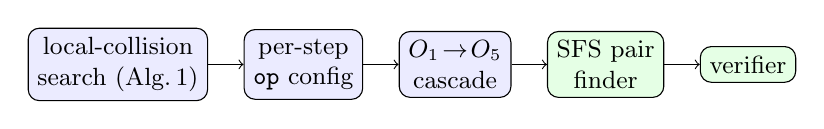
\begin{tikzpicture}[node distance=0.45cm, every node/.style={font=\small, align=center}]
\node[draw, rounded corners, fill=blue!8] (lc) {local-collision\\search (Alg.\,1)};
\node[draw, rounded corners, right=of lc, fill=blue!8] (cfg) {per-step\\\texttt{op} config};
\node[draw, rounded corners, right=of cfg, fill=blue!8] (cas) {$O_1\!\to\!O_5$\\cascade};
\node[draw, rounded corners, right=of cas, fill=green!10] (fc) {SFS pair\\finder};
\node[draw, rounded corners, right=of fc, fill=green!10] (vf) {verifier};
\draw[->] (lc)--(cfg); \draw[->] (cfg)--(cas); \draw[->] (cas)--(fc); \draw[->] (fc)--(vf);
\end{tikzpicture}
\begin{itemize}
  \item To check the pipeline: we drove it on the 24-step Sanadhya--Sarkar local collision $[10,11,12,13,17,18]$ and produced a \key{verified} semi-free-start colliding pair (next slide). However, this setup is not ideal for smaller rounds.
  \item Pinning the per-step trail (a guided solve) found it in $\sim$23\,s.
\end{itemize}
\end{frame}

\begin{frame}{Our 24-step SHA-256 result (SS local collision)}
\textbf{Differential characteristic} ($O_3=1$, i.e.\ $\Pr=2^{-1}$; active region steps 10--18):
\begin{block}{}
\centering\ttfamily\footnotesize
\begin{tabular}{r l l l}
$i$ & $\nabla A_i$ & $\nabla E_i$ & $\nabla W_i$\\
10 & =========================unnnnnn & ==unnnnnnnnnnnnnnnnnnnnnnnnnnnnn & ===============================u\\
11 & ================================ & =u====u=u=u=u=n==u===u========u= & ===============================n\\
12 & ================================ & =============================n== & =================nn=============\\
13 & ================================ & uuuuuuuuuuuuuuuuuuuuuuuuuuuuuuu= & ==================n=============\\
14 & ================================ & ===============================u & ================================\\
15 & ================================ & ================================ & ================================\\
16 & ================================ & ================================ & ================================\\
17 & ================================ & ================================ & ===============================u\\
18 & ================================ & ================================ & ==============================nu\\
\end{tabular}
\end{block}
\small $O_3=1$ here is a single \key{Boolean (IF) condition}.
\textbf{Verified semi-free-start colliding pair} (differs only in input words $\{10,11,12,13\}$; words $17,18$ from expansion):
\begin{block}{}
\centering\ttfamily\small
CV\_in: b75feccb 293d0b0c d66d41be d8050e1f 8cc675b4 0997b9ac cbeb9f5e 7a55becd\\[3pt]
M\ \ (W10..W13): 6ff4b62\hot{d} \ c0f6e38\hot{a} \ 35aa\hot{0}8b5 \ 9d9e\hot{9}c9a\\[2pt]
M'\ (W10..W13): 6ff4b62\hot{c} \ c0f6e38\hot{b} \ 35aa\hot{6}8b5 \ 9d9e\hot{b}c9a
\end{block}
\end{frame}

\begin{frame}{A caution on generalizability}
\begin{itemize}
  \item The objective minimizes the \key{message}-difference weight; a sparse local collision can still be \emph{state}-dense (high $O_3$). At reduced rounds, sparsity-ranked collisions give useless $O_3$ (e.g.\ $32,91$ for $R=22,24$).

  \item \key{The method is built for long rounds.} Algorithm 1's ``good LC'' conditions and the message-weight$\leftrightarrow$state-cancellation alignment hold in the $R\approx 32$--$37$ regime; at short rounds they diverge.
\end{itemize}
\centering\emph{Long-round, high-probability local collisions are where this approach pays off; short rounds need state-aware selection.}
\end{frame}

% =====================================================================
\section{Message modification}

\begin{frame}{Message modification: the control horizon and two blocks}
\textbf{Why it is mandatory.} Naively a DC costs $2^{\#\text{conditions}}\gg 2^{128}$; worse than birthday. Message modification satisfies conditions \emph{deterministically} using message freedom.
\begin{block}{The control horizon}
\small Solving the state equation for the message word, $W_i = E_i\bsub A_{i-4}\bsub E_{i-4}\bsub\Sigma_1(E_{i-1})\bsub\mathrm{IF}(\cdot)\bsub K_i$, means: \emph{fix the early state $\Rightarrow$ the $W_i$ are determined}. Conditions in steps $\le 15$ are \key{free}; $W_{\ge 16}$ are expansion-forced $\Rightarrow$ control ends at step 15. Split: controlled ($\le 15$) $+$ \key{uncontrolled} ($\ge 16$, count $=\beta$).
\end{block}
\textbf{From SFS to a real collision (two-block).} An SFS attack needs a \emph{free} chaining value $CV_1$ to dial in early state; the true IV gives a fixed one. \key{Use a first block $M_0$ to randomize $CV_1$}: collide in block 2, vary $M_0$ until $CV_1$ is usable. (Mendel'13 / Li'24.)
\end{frame}

\begin{frame}{Two-block}
\begin{block}{The non-obvious core}
\small \key{Pre-compute a table} of ``good'' chaining-value prefixes (by solving the dense early part of the trail), indexed by a $A_{-1}$. Keep resampling $M_0$ until $A_{-1}$ word matches a table entry; the rest of $CV_1$ is absorbed \emph{deterministically} by deriving the missing state/message words. The 8 chaining words split as \key{absorb 7, match 1}.
\end{block}
\begin{itemize}\small
  \item Match cost $\sim 2^{32}/|\text{table}|$; everything after the match is forced, then the $\beta$ uncontrolled conditions are checked.
  \item \textbf{37-step SHA-256:} pre-processing $\sim$7 days; $\beta\approx 95$; $T\approx 2^{122.2}$ (match $A_{-1}$), improved to \textcolor{key}{$\mathbf{2^{119.1}}$} by matching $(A_{-2},A_{-1})$, memory $2^{34.9}$--$2^{39.9}$. (36-step: $2^{94.4}$.)
\end{itemize}
\end{frame}

% =====================================================================
\section{Further work}

\begin{frame}{Suggested further work}
\begin{itemize}
  \item \key{Port the 2026 machinery to SHA-512}; the complete/variable-specific Boolean models and the local-collision tool were shown on SHA-256; SHA-512 lags (28 practical / 31 theoretical).
  \item \key{Better / longer local collisions}; the explicit 2026 motivation: more steps come first from a better message-expansion local collision.
\end{itemize}
\end{frame}

\end{document}
